% include the figures path relative to the master file
\graphicspath{ {./content/method/figures/} }

\section{Data}\label{sec:data}

The datasets used in this study were acquired by the \gls{seri}, using CIRRUS TM (Carl Zeiss Meditec, Inc., Dublin, CA) \gls{sdoct} device~\cite{Chen2005}.
The datasets consist of 32 \gls{oct} volumes (16 \gls{dme} and 16 normal cases).
Each volume contains 128 B-scan with resolution of 512~$\times$~1024 pixels.
All \gls{sdoct} volumes are read and assessed by trained graders and identified as normal or \gls{dme} cases based on evaluation of retinal thickening, hard exudates, intraretinal cystoid space formation and subretinal fluid as presented in the table below.
Within the \gls{dme} dataset, a large number of lesions were selected to create a rather complete \gls{dme} dataset.
The volumes and sample numbers for each volume are presented below (Fig.\,\ref{fig:bbdd}):

\begin{figure*}[t]
\centering
        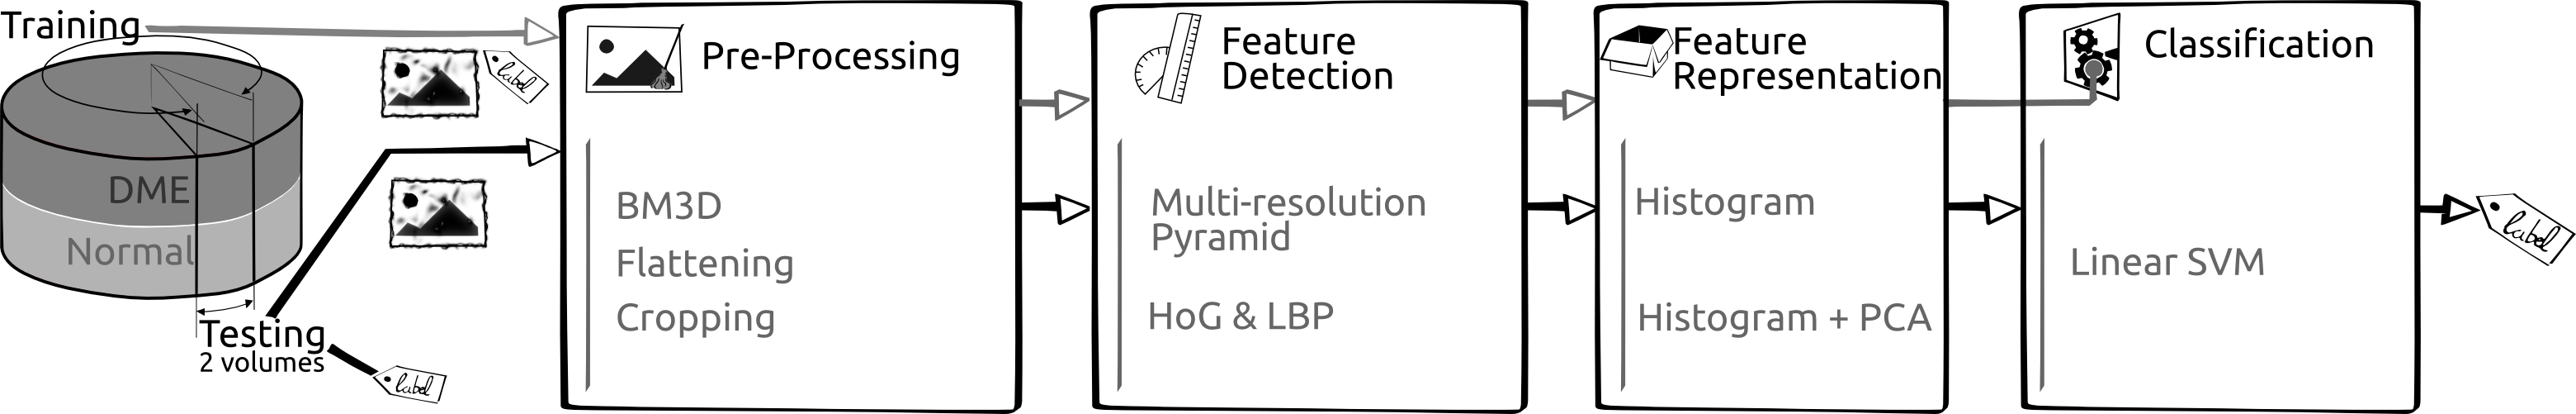
\includegraphics[width = 0.98\textwidth]{khaled_embc}
\caption{Proposed classification pipeline}
\label{fig:fig3}
\end{figure*}

